\textbf{Visning af spilleplade}
\begin{figure}%[thp]
%  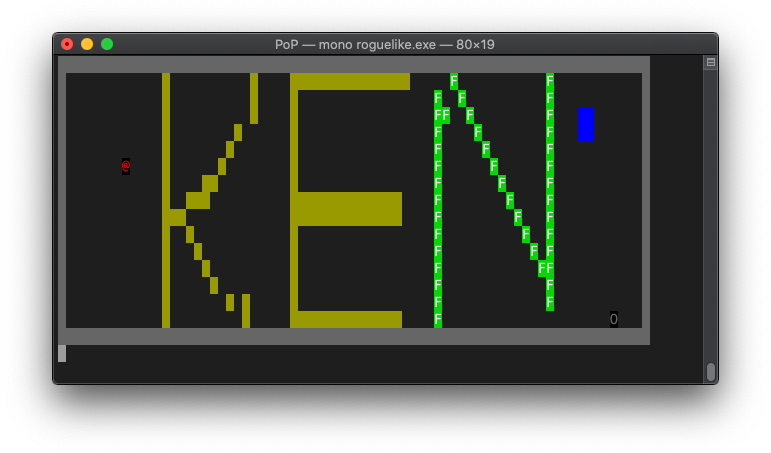
\includegraphics[width=.99\linewidth]{screenshot.png}
  \begin{center}
    \begin{minipage}{5cm}
\begin{verbatim}
+--+--+--+--+--+--+--+
|BB                  |
+  +  +  +--+--+  +  +
|      AA|           |
+  +  +--+  +  +  +  +
|               gg   |
+  +  +  +  +  +  +  +
|                  CC|
+--+--+--+--+--+--+--+
\end{verbatim}
    \end{minipage}
  \end{center}
  \caption{Eksempel på visning af spilleplade.}
  \label{fig:example-text}
\end{figure}

For at kunne vise en spilleplade implementerer vi en klasse
\lstinline{BoardDisplay}, som er et gitter af felter. Hvor feltet
i øverste ventre hjørne har position $(1,1)$, og første koordinat
tælles op når man bevæger sig
fra nord til syd (top mod bund) og anden koordinat tælles op fra vest mod øst.

En plade har altid alle ydre vægge. For at håndtere indre vægge, så
kan hver felt have en nedre væg og en højre væg, men ikke andre vægge.
Hvert felt kan vise en tekststreng på maksimalt to tegn. Se
Figur~\ref{fig:example-text} for at se en visning af spillet fra
Figur~\ref{fig:example}.

Implementér klassen \lstinline{BoardDisplay} med følgende signatur:

\begin{lstlisting}
type BoardDisplay =
  class
    new : rows:int * cols:int -> BoardDisplay
    member Set : x:int * y:int * cont:string -> unit
    member SetBottomWall : x:int * y:int -> unit
    member SetRightWall : x:int * y:int -> unit
    member Show : unit -> unit
  end
\end{lstlisting}

Det vil sige:
\begin{itemize}
\item En konstruktør der tager antal rækker og koloner som argumenter.
\item en metode \lstinline{Set} til at sætte indhold i et
  felt.
\item to metoder \lstinline{SetBottomWall} og \lstinline{SetRightWall}
  til at sætte indre vægge for et
  felt.
\item en metode \lstinline{Show} til at vise en canvas i
  terminalen.
\end{itemize}

I rapporten skal I beskrive jeres designovervejelser, samt redegøre
for hvilke data klassen \lstinline{BoardDisplay} har.

% \textbf{Hints}: Til \lstinline{Show} skal I bruge følgende
% funktionalitet fra standard-biblioteket:

% \begin{itemize}
% \item \lstinline{System.Console.ForegroundColor <- System.ConsoleColor.White}
%   til at sætte forgrundsfarven til hvid
%   (kan også bruges til andre farver).
% \item \lstinline{System.Console.BackgroundColor <- System.ConsoleColor.Blue}
%   til at sætte baggrundsfarven til blå
%   (kan også bruges til andre farver).
% \item \lstinline{System.Console.ResetColor()} til at sætte farverne i
%   terminalen tilbage til normal.
% \end{itemize}


%%% Local Variables:
%%% mode: latex
%%% TeX-master: "main"
%%% End:
